\documentclass[tikz,border=4pt]{standalone}
\usepackage{amsmath,amssymb}
\usepackage{pgfplots}
\pgfplotsset{compat=1.18}
\usepgfplotslibrary{fillbetween}
\usetikzlibrary{arrows.meta,calc}
% altitude-map colour: green (low F) -> yellow -> brown (high F)
\newcommand{\fcol}[1]{%
  \pgfmathsetmacro{\fv}{#1}%
  \ifdim\fv pt<50pt
    \pgfmathsetmacro{\fw}{2*\fv}\colorlet{fc}{Fmid!\fw!Flo}%
  \else
    \pgfmathsetmacro{\fw}{2*(\fv-50)}\colorlet{fc}{Fhi!\fw!Fmid}%
  \fi}
\colorlet{Flo}{green!50!black}
\colorlet{Fmid}{yellow!90!orange}
\colorlet{Fhi}{brown!85!black}
\begin{document}
% ------------------------------------------------------------------
% Grid argument on the simplex of spectra alpha=(a1,a2,a3), d_A = 3.
% One-column layout (~7.5 cm wide): (a) on top, (b) below.
% Coordinates: alpha -> a1*A + a2*B + a3*C, with
% A=(0,0), B=(\S,0), C=(\S/2,\H), \S = side length, \H = sqrt(3)/2 \S.
% ------------------------------------------------------------------
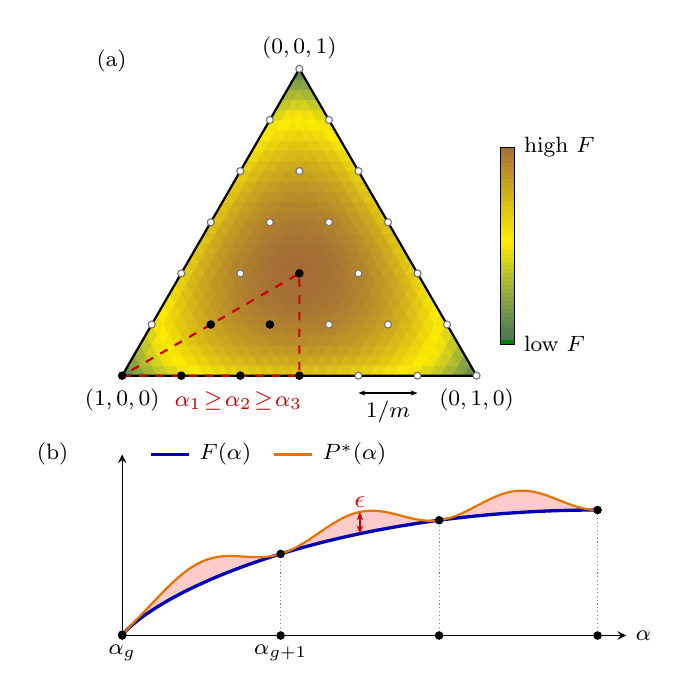
\begin{tikzpicture}[
    every node/.style={font=\footnotesize},
    gp/.style={circle,fill=black,inner sep=1.1pt},
    gpo/.style={circle,draw=black!55,fill=white,inner sep=0.9pt},
  ]
  \def\N{30}      % resolution of the colour map
  \def\M{6}       % resolution of the grid G
  \def\S{4.5}     % side length of the simplex (cm)
  \pgfmathsetmacro{\H}{0.8660254*\S}
  % ---------- (a) colour map of F on the simplex ----------
  \foreach \i in {0,...,29}{
    \pgfmathtruncatemacro{\jmax}{\N-1-\i}
    \foreach \j in {0,...,\jmax}{
      % upward triangle, colour from centroid
      \pgfmathsetmacro{\b}{(\i+1/3)/\N}\pgfmathsetmacro{\c}{(\j+1/3)/\N}
      \pgfmathsetmacro{\a}{1-\b-\c}
      \pgfmathsetmacro{\F}{100*(-\a*ln(\a)-\b*ln(\b)-\c*ln(\c))/ln(3)}
      \fcol{\F}\fill[fc,draw=fc,line width=0.2pt]
        ({\S*(\i+\j/2)/\N},{\H*\j/\N}) --
        ({\S*(\i+1+\j/2)/\N},{\H*\j/\N}) --
        ({\S*(\i+(\j+1)/2)/\N},{\H*(\j+1)/\N}) -- cycle;
      % downward triangle
      \ifnum\j<\jmax
        \pgfmathsetmacro{\b}{(\i+2/3)/\N}\pgfmathsetmacro{\c}{(\j+2/3)/\N}
        \pgfmathsetmacro{\a}{1-\b-\c}
        \pgfmathsetmacro{\F}{100*(-\a*ln(\a)-\b*ln(\b)-\c*ln(\c))/ln(3)}
        \fcol{\F}\fill[fc,draw=fc,line width=0.2pt]
          ({\S*(\i+1+\j/2)/\N},{\H*\j/\N}) --
          ({\S*(\i+1+(\j+1)/2)/\N},{\H*(\j+1)/\N}) --
          ({\S*(\i+(\j+1)/2)/\N},{\H*(\j+1)/\N}) -- cycle;
      \fi
    }
  }
  % simplex boundary
  \draw[thick] (0,0) -- (\S,0) -- (\S/2,\H) -- cycle;
  % ordered chamber a1 >= a2 >= a3
  \draw[thick,red!80!black,dashed] (0,0) -- (\S/2,0) -- (\S/2,\H/3) -- cycle;
  % grid G (filled: inside the chamber; hollow: fixed by symmetry)
  \foreach \i in {0,...,6}{
    \pgfmathtruncatemacro{\jmax}{\M-\i}
    \foreach \j in {0,...,\jmax}{
      \pgfmathtruncatemacro{\k}{\M-\i-\j}
      \pgfmathtruncatemacro{\inch}{(\k>=\i)&&(\i>=\j)}
      \ifnum\inch=1
        \node[gp]  at ({\S*(\i+\j/2)/\M},{\H*\j/\M}) {};
      \else
        \node[gpo] at ({\S*(\i+\j/2)/\M},{\H*\j/\M}) {};
      \fi
    }
  }
  % spacing between neighbouring grid points
  \draw[{Stealth[length=2.5pt]}-{Stealth[length=2.5pt]},thick]
    ({4*\S/6},-0.22) -- ({5*\S/6},-0.22) node[midway,below=-1pt] {$1/m$};
  % vertex labels
  \node[below] at (0,-0.05)         {$(1,0,0)$};
  \node[below] at (\S,-0.05)        {$(0,1,0)$};
  \node[above] at (\S/2,\H)         {$(0,0,1)$};
  \node[red!80!black,anchor=north] at (\S/4+0.35,-0.08)
    {$\alpha_1\!\geq\!\alpha_2\!\geq\!\alpha_3$};
  \node[anchor=west] at (-0.45,\H+0.1) {(a)};
  % colour bar
  \foreach \t in {0,2,...,98}{
    \fcol{\t}\fill[fc] ({\S+0.3},{0.4+0.025*\t}) rectangle ({\S+0.48},{0.4+0.025*\t+0.06});
  }
  \draw ({\S+0.3},0.4) rectangle ({\S+0.48},2.9);
  \node[right] at ({\S+0.48},0.4) {low $F$};
  \node[right] at ({\S+0.48},2.9) {high $F$};

  % ---------- (b) 1D cut along the chamber edge (1,0,0) -> (1/2,1/2,0) ----------
  \begin{axis}[
      at={(0cm,-3.3cm)}, anchor=south west,
      width=6.4cm, height=2.3cm, scale only axis,
      axis lines=left, xmin=0, xmax=0.53, ymin=0, ymax=1.0,
      xtick=\empty, ytick=\empty, xlabel={$\alpha$},
      xlabel style={at={(1,0)},anchor=west},
      clip=false, samples=200, domain=0.0005:0.5,
      declare function={F(\t)=-\t*ln(\t)-(1-\t)*ln(1-\t);
                        ep=0.12;
                        P(\t)=F(\t)+ep*sin(6*180*\t)^2;}]
    % F along the cut (binary entropy)
    \addplot[very thick,blue!70!black,name path=Fp] {F(x)};
    % illustrative P*: P* <= F on the grid, exceeds F by at most eps in between
    \addplot[thick,orange!90!black,name path=Pp] {P(x)};
    % shade the overshoot P* - F between grid points
    \addplot[red!60,opacity=0.35] fill between[of=Pp and Fp];
    % grid points
    \foreach \t in {0,1,2,3}{
      \edef\tmp{\noexpand\draw[densely dotted,black!50]
        (axis cs:\t/6,0) -- (axis cs:\t/6,{F(max(\t/6,0.0005))});
        \noexpand\node[gp] at (axis cs:\t/6,{F(max(\t/6,0.0005))}) {};
        \noexpand\node[gp] at (axis cs:\t/6,0) {};}\tmp
    }
    \node[below] at (axis cs:0,0)   {$\alpha_{g}$};
    \node[below] at (axis cs:1/6,0) {$\alpha_{g+1}$};
    % epsilon marker at a maximal bump
    \draw[{Stealth[length=3pt]}-{Stealth[length=3pt]},thick,red!80!black]
      (axis cs:0.25,{F(0.25)}) -- (axis cs:0.25,{P(0.25)});
    \node[red!80!black,font=\small,anchor=south,inner sep=1.5pt]
      at (axis cs:0.25,{P(0.25)}) {$\epsilon$};
    % legend
    \draw[very thick,blue!70!black] (axis cs:0.03,1.0) -- (axis cs:0.07,1.0)
      node[right,black] {$F(\alpha)$};
    \draw[thick,orange!90!black]    (axis cs:0.16,1.0) -- (axis cs:0.20,1.0)
      node[right,black] {$P^*(\alpha)$};
    \node[anchor=west] at (axis cs:-0.1,1.0) {(b)};
  \end{axis}
\end{tikzpicture}
\end{document}